\documentclass[conference]{IEEEtran}
\IEEEoverridecommandlockouts
% The preceding line is only needed to identify funding in the first footnote. If that is unneeded, please comment it out.
\usepackage{cite}
\usepackage{amsmath,amssymb,amsfonts}
\usepackage{algorithmic}
\usepackage{graphicx}
\usepackage{textcomp}
\usepackage{xcolor}
% My packages start
\usepackage{hyperref}
\usepackage{glossaries}
\usepackage{cleveref} % Reference footnotes.
\crefformat{footnote}{#2\footnotemark[#1]#3}
% TODO: Use flushend if needed.
% \usepackage{flushend} % Balances columns on the last page.

\newacronym{jive}{JIVE}{Java Interactive Visualization Environment}
\newacronym{uml}{UML}{Unified Modeling Language}
\newacronym{ide}{IDE}{Integrated Development Environment}
\newacronym{api}{API}{Application Programming Interface}
\newcommand{\intellij}{IntelliJ IDEA}
\newcommand{\screencast}{\url{https://www.youtube.com/}}
% My packages end

\def\BibTeX{{\rm B\kern-.05em{\sc i\kern-.025em b}\kern-.08em
    T\kern-.1667em\lower.7ex\hbox{E}\kern-.125emX}}
\begin{document}

\title{The Visual Debugger Tool\\
{}
\thanks{}
}

\author{\IEEEauthorblockN{
% 1\textsuperscript{st}
Tim Kräuter}
\IEEEauthorblockA{
% \textit{Department of Computer science,} \\
% \textit{Electrical engineering and Mathematical sciences} \\
\textit{Høgskulen på Vestlandet}\\
Bergen, Norway \\
tkra@hvl.no}
% \and
% \IEEEauthorblockN{
% % 2\textsuperscript{nd}
% Adrian Rutle}
% \IEEEauthorblockA{
% % \textit{Department of Computer science,} \\
% % \textit{Electrical engineering and Mathematical sciences} \\
% \textit{Høgskulen på Vestlandet}\\
% Bergen, Norway \\
% aru@hvl.no}
% \and
% \IEEEauthorblockN{
% % 3\textsuperscript{rd}
% Harald König}
% \IEEEauthorblockA{
% % \textit{Department of Computer science,} \\
% % \textit{Electrical engineering and Mathematical sciences} \\
% \textit{University of Applied Sciences, FHDW}\\
% Hannover, Germany \\
% harald.koenig@fhdw.de}
% \and
% \IEEEauthorblockN{
% % 4\textsuperscript{th}
% Yngve Lamo}
% \IEEEauthorblockA{
% % \textit{Department of Computer science,} \\
% % \textit{Electrical engineering and Mathematical sciences} \\
% \textit{Høgskulen på Vestlandet}\\
% Bergen, Norway \\
% yla@hvl.no}
}

\maketitle

% TODO: 3-5 Minute screen cast showcasing the tool (Put it on youtube, Maybe with my developer account). Also link that one in the abstract and on the plugin page.
% 4 pages + 1 page of only references!

\begin{abstract}
\emph{Debugging} is an important activity in software development to understand control- and data flow in the source code.
Understanding the source code is a prerequisite to finding and fixing bugs or implementing new desired features. 
Traditionally information during program runtime is visualized in a textual manner while debugging.
However, we have developed a novel tool for visualizing program information as object diagrams, which is integrated as a plugin into the popular Java development environment \intellij{}.
Our tool is demonstrated in a typical usage scenario here\footnote{\screencast}.
\end{abstract}

\begin{IEEEkeywords}
Debugging, Visual Debugging, Visual Debugger, Software Visualization, IntelliJ IDEA Plugin
\end{IEEEkeywords}

\section{Introduction}
% Introduce debugging
Debugging is an essential part of software maintenance and evolution since it allows a software developer to halt the execution of a program at any point to analyze the current program state.
% Describe why debugging is important/ some typical usage scenarios

% Debugging works on a textual representation of the software
Traditionally program information is represented in a textual manner during debugging, see \autoref{fig:variablesIntellij}.

% Motivation
% Software developers spend a lot of time on debugging
Moreover, software developers spend between 35 and 50 percent of their time validating and debugging software \cite{odellDebuggingMindsetUnderstanding2017}.
However, a graphical representation might allow for a faster and better understanding of specific scenarios.
% Make debugging more efficient by a better visualization of the debugging data
Thus, research to visualize program information graphically during debugging has started, motivated by possible reductions in the time spent during debugging. 

% Introduce my plugin:
% Integrated in the most popular JAVA-IDE according to some report
% Visualize program state graphically using object diagrams
We have developed an \intellij{} plugin\footnote{The plugin can be found at \url{https://plugins.jetbrains.com/plugin/16851-visual-debugger}.}, which visualizes the program state as an object diagram for better program comprehension.
% Explain the plugin shortly and link to a YouTube video. 

% Paper outline
The remainder of this paper is structured as follows.
We describe the visual debugger tool in detail (\autoref{sec:toolDescription}) before explaining the tool architecture (\autoref{sec:architecture}).
Finally, we discuss related work in \autoref{sec:relatedWork} and conclude in \autoref{sec:conclusion}.

\section{Tool description} \label{sec:toolDescription}
We will describe our tool using the parts list model shown in \autoref{fig:partsListModel}.
\begin{figure}[h]
    \centering
    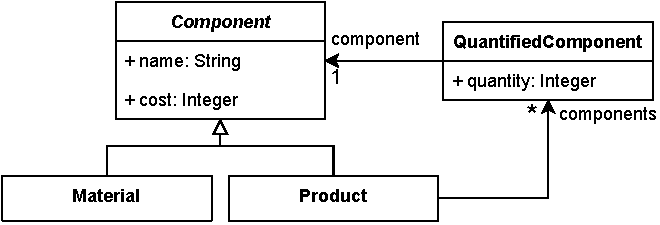
\includegraphics[width=0.48\textwidth]{images/VD-parts list class diagram.pdf}
    \caption{Parts list class diagram}
    \label{fig:partsListModel}
\end{figure}

Program information during debugging is usually represented \textit{textually} in \glspl*{ide}.
For example, \autoref{fig:variablesIntellij} shows objects during debugging in \intellij{} conforming to the parts list model. 

\begin{figure}[h]
    \centering
    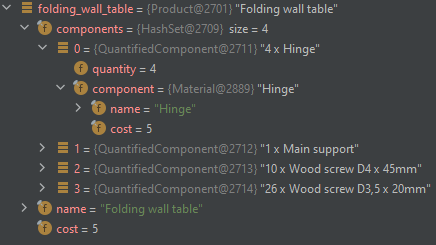
\includegraphics[width=0.4\textwidth]{images/variables.png}
    \caption{Variables during debugging in \intellij}
    \label{fig:variablesIntellij}
\end{figure}

We have unfolded the substructure of the \textsf{folding wall table} object to see its components and first component in detail.
If one is not only interested in one attribute inside one object, but rather the whole object world using the textual representation is cumbersome.

Consequently, research on visual debugging began with the goal of fostering program comprehension.
Our tool is one of many visual debugging tools, but we aimed for excellent usability by seamlessly integrating our tool in the debugging process of the \intellij{}.
In addition, our tool is straightforward and non-intrusive, i.e., it complements textual debugging.
The goal of our tool is to make debugging during software development as efficient as possible to increase software developer productivity.

Using our visual debugger tool, we obtain the object diagram\footnote{\label{footnote:artifacts} Source code, a screencast demonstrating the visual debugger tool and more can be found at \url{https://github.com/timKraeuter/ICSME-2022}.} shown in \autoref{fig:visualDebuggerVariables}, which contains the same objects and level of detail as \autoref{fig:variablesIntellij}.

\begin{figure}[h]
    \centering
    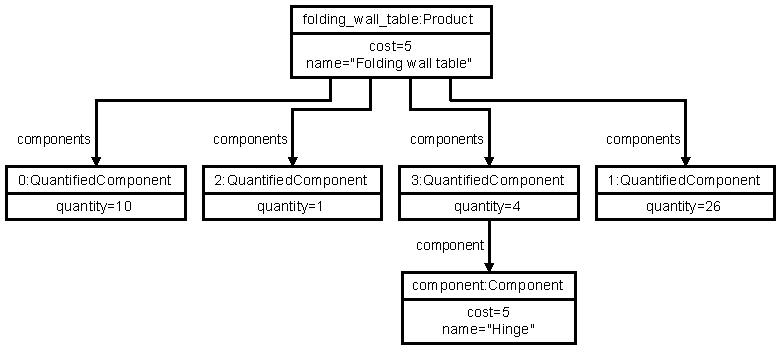
\includegraphics[width=0.48\textwidth]{images/VD-parts list object diagram.pdf}
    \caption{Visual Debugger visualization comparable to \autoref{fig:variablesIntellij}}
    \label{fig:visualDebuggerVariables}
\end{figure}

% Object diagram visualization
The visual debugger tool continuously visualizes the variables in the scope of the debugging session as an \textit{object diagram}.
The visualization starts automatically when the first breakpoint is reached during debugging if the visual debugger tool is activated.
Thus, if desired, a software developer can use the visual debugger alongside the textual debugging view.
The visualization is always up to date since we listen to the events generated by a debugging session in \intellij{}.
Consequently, we update the visualization whenever a new breakpoint is reached, or a user steps through the program code.

% Interaction by double clicking on an object will load all directly linked objects
Textual debugging views only show the root objects (directly referenced in the debugging session) without attributes when debugging is started.
% Initial visualization depth
Similarly, we also do not visualize all objects linked to the root objects, but we allow the user to configure a \textit{visualization depth}.
The visualization depth describes how many links starting from the root objects should be followed to find objects for the initial visualization.
Afterward, one can explore objects further by double-clicking them in the visualization just as one would double-click objects in the textual debugger.
For example, in \autoref{fig:visualDebuggerVariables}, one quantified component was explored further.
The visualization is browser-based and implemented in a standalone \textit{visualization component}, which automatically layouts the object diagram using the Eclipse Layout Kernel.
% Embedded visualizer without interaction
In addition, we provide a visualization based on PlantUML embedded in \intellij{}.
However, it is not possible to explore objects inside the embedded visualization since PlantUML provides static \gls*{uml} diagrams.

% Describe the functionality of the tool, downloads, mention components. Maybe some contributions/differences to other tools?

% State how many downloads we have atm
The visual debugger tool has 1804 unique downloads\footnote{Last checked on March 8, 2022, see \url{https://plugins.jetbrains.com/plugin/16851-visual-debugger}.} and positive reviews.
It consists of two components, namely the debugging and the visualization component, which we will describe in more detail in the tool architecture section.

\section{Tool architecture}  \label{sec:architecture}
First, the \textit{debugging component} integrates with \intellij{} by automatically hooking into all started debugging processes of the \gls*{ide}.
The goal of the debugging component is to obtain the current debugging information from \intellij{} and pass it on to the visualization component.
In addition, the debugging component offers a method to load detailed information for individual objects in the current debugging scope, as described earlier.

Second, the \textit{visualization component} represents the debugging information as an object diagram to ease program understanding.
Moreover, it allows interaction to load additional debugging information for the currently shown objects.
The visualization component is \emph{browser-based} and relies on a fixed \emph{Visual Debugging \gls*{api}}.
Consequently, we could implement a debugging component for a different \gls*{ide}, such as Eclipse, and reuse the visualization component.
Furthermore, the visualization component is independent of the underlying object-oriented programming, in our case Java, and could even be reused in a visual debugger for other  languages.

% Explain the Debugging API
The \textit{Visual Debugging \gls*{api}}\cref{footnote:artifacts} is based on \emph{WebSocket} to allow live updates about changes in the debugging information, see \autoref{fig:api}.

\begin{figure}[h]
    \centering
    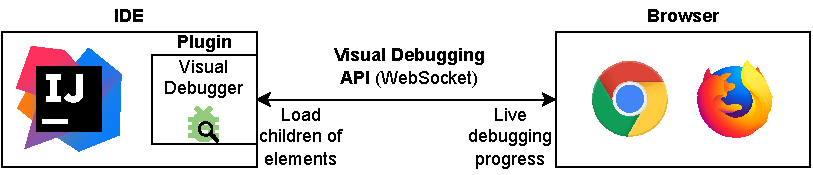
\includegraphics[width=0.488\textwidth]{images/VD-architecture.pdf}
    \caption{Communication through the Debugger API}
    \label{fig:api}
\end{figure}

Initially, a browser connects to the WebSocket server hosting the Debugger \gls*{api}, for example the server included in our Visual Debugger plugin.
Afterward, the browser is updated in real-time about new debugging information due to debugging actions in the \gls*{ide}, such as hitting a breakpoint or jumping to the next line in the source code.
In addition, the visualization component allows a user to interact with the visualization to load all direct children and attributes of any shown object.
Both components are open-source\cref{footnote:artifacts} and put together result in the visual debugger tool.

\section{Related work} \label{sec:relatedWork}
Visual debugging has been researched since the 90s \cite{baeza-yatesVisualDebuggingAutomatic1996, jerdingUsingVisualizationFoster1994, mukherjeaVisualDebuggingIntegrating1994, hansonSimpleExtensibleGraphical1997}, but most of the resulting tools are outdated by now.
We will now describe some recent visual debugging tools and compare them to our tool.

% JIVE is comprehensive but the downside is that it offers too much functionality!
\textit{\gls*{jive}}\footnote{\url{https://cse.buffalo.edu/jive/}} is a plugin for the Eclipse \gls*{ide} \cite{czyzDeclarativeVisualDebugging2007,k.p.FiniteStateModel2021}.
It provides interactive Java program execution visualization at different levels of granularity.
The program state is visualized as a \gls*{uml} object diagram, while the call stack is represented as a \gls*{uml} sequence diagram.
\gls*{jive} is tightly coupled to the Eclipse \gls*{ide} and does not integrate with Eclipses debugger but rather is a debugging environment on its own.
This approach is a significant difference to our tool, which integrates with the debugging tool of the \gls*{ide}.
It makes \gls*{jive} powerful but complex since it is hard to understand what is going on in the multiple views provided by \gls*{jive}.
Compared to \gls*{jive} the visual debugger tool focuses only on object diagram visualization, which makes it lightweight and straightforward to use.
In addition, our tool decouples debugging and visualization, such that it can be adopted to different \glspl*{ide} even based on other object-oriented programming languages than Java.

% Java Visualizer
A plugin called \textit{Java Visualizer}\footnote{\url{https://plugins.jetbrains.com/plugin/11512-java-visualizer}} has been developed for the \intellij{}.
It visualizes the call stack and objects contained in the Java heap as a box-and-pointer diagram during a debugging session.
However, even in simple scenarios, the visualized call stacks are long since all objects from the Java heap are visualized and not only the variables in the debugging scope.
This leads to much noise in the visualization, especially if one is only interested in the current objects, i.e., the current system state.
This plugin inspired us, but our tool tries to improve by showing not all the present information and allowing a user to load more relevant information if needed.

% Debugging for distributed applications
In \cite{kochGraphicalDebuggingDistributed2015}, the authors describe a tool to debug distributed applications.
It can connect to multiple Java virtual machines and show the retrieved objects separately in an object diagram or combine the same objects from different JVMs using object identifiers or other properties.
The tool is also tightly integrated with the Eclipse \gls*{ide} and tackles the problem of debugging distributed applications, which we do not address.
However, we could not find and test the tool by ourselves.
In the future, we could incorporate these ideas by allowing multiple debugging components (one for each application) to connect to one visualization component.
The visualization component can then show the different debugging views separately or combined as described in \cite{kochGraphicalDebuggingDistributed2015}.

\textit{JAVAVIS} is a standalone tool to help students understand program execution in Java \cite{oechsleJAVAVISAutomaticProgram2002}.
It makes use of object- and sequence diagrams to represent program behavior.
However, it is not integrated with modern \glspl*{ide} such as Eclipse or \intellij{}.
Our tool can also be used to help students to learn Java or object-oriented program execution, but we currently do not provide a sequence diagram visualization.

\section{Conclusion \& future work} \label{sec:conclusion}
% Conclude
Contributions:
\begin{enumerate}
    \item My work is integrated with a modern, highly popular (most popular) \gls*{ide} for Java Development. (+ open-source and downloaded many times already)
    \item Visualization is independent and can be reused for debugging any object-oriented software by implementing the fixed debugging API.
    \item Usability and up to date. Other tools are highly academic and do a lot but too much for practical usage scenarios. Our focus is on software developers.
    \item Interaction with the generated object diagrams?
\end{enumerate}

% Future work based on the plugin

% Future work somehow connecting to my main line of research?
\cite{krauterBehavioralConsistencyHeterogeneous2021}

\section*{Acknowledgment}

\newpage

% TODO: check References one by one at the end!
\bibliographystyle{IEEEtran}
\bibliography{bib}

\end{document}
